\documentclass{article}

\usepackage[utf8]{inputenc} 
\usepackage[T1]{fontenc}
\usepackage[french]{babel}
\usepackage[margin=2.5cm]{geometry}
\usepackage{hyperref}
\usepackage{graphicx}
\usepackage[ruled,linesnumbered]{algorithm2e}
\usepackage{xcolor}
\usepackage{amsmath}
\usepackage{amssymb}

\newcommand{\pluseq}{\mathrel{+}=}
\newcommand{\minuseq}{\mathrel{-}=}
\newcommand\comm[1]{\footnotesize\ttfamily\textcolor{gray}{// #1}}

\title{Projet C++ : problème du sac à dos à choix multiple et politique d'incitations}
\author{\textsc{Javaudin} Lucas, \textsc{Le Rest} François}

\begin{document}

\maketitle

\tableofcontents

\newpage

\section{Introduction}

En recherche opérationnelle, le problème du sac à dos\footnote{Voir \url{en.wikipedia.org/wiki/Knapsack_problem}} est un problème d'optimisation dont l'objectif est de maximiser la valeur des objets que l'on insère dans un sac qui ne peut pas supporter plus d'un certain poids.

Nous étudions ici une variante du problème du sac à dos : le problème du sac à dos à choix multiple ou \textit{multiple choice knapsack problem} (MCKP).
Dans le MCKP, les objets sont regroupés en plusieurs classes et le sac à dos doit être rempli avec un et un seul objet de chaque classe.

Le MCKP est un problème NP-complet.
Nous proposons plusieurs algorithmes qui donnent une approximation de la solution optimale.
Plus précisément, les solutions proposées par ces algorithmes sont réalisables et leur distance par rapport à la solution optimale est bornée.

Enfin, nous montrons que le problème du sac à dos à choix multiple est équivalent au problème consistant à trouver la politique d'incitations maximisant l'utilité sociale, lorsque les individus font face à un choix discret et lorsque le budget de la politique est contraint.

\section{Algorithmes}
% On peut mettre ici un pseudo-code des algorithmes que l'on a codé.

\subsection{Recherche exhaustive}

L'algorithme de recherche exhaustive parcourt toutes les allocations possibles et renvoie l'allocation optimale, c'est-à-dire l'allocation qui a la plus grande valeur parmi toutes les allocations dont le poids ne dépasse pas la capacité du sac à dos.

Cet algorithme est NP-hard.
En effet, si l'on note $J$ le nombre de classes et $n$ le nombre d'objets dans chaque classe, alors le nombre d'allocation possible est $n^J$.\footnote{Nos algorithmes autorisent un nombre d'objets différent dans chaque classe. Dans ce cas, le nombre d'allocation possible est $n_1 \cdot \dots \cdot n_J$ où $n_i$ est le nombre d'objets dans la classe $i$.}

Pour parcourir toutes les allocations, on ordonne les objets dans chaque classe et on commence par l'allocation qui prend le premier objet de chaque classe.
Pour obtenir l'allocation suivante, on prend l'objet suivant de la première classe.
Si l'on atteint le dernier objet de la première classe, alors on prend l'objet suivant de la deuxième classe (si ce n'est pas le dernier de la classe), et ainsi de suite.
La table \ref{tab:recherche-exhaustive} montre comment l'algorithme parcourt toutes les allocations lorsque qu'il y a trois classes avec trois objets dans chaque classe (les objets sont indicés 0, 1 et 2).

\begin{table}[!ht]
	\centering
	\caption{Fonctionnement de la recherche d'allocation pour $J=3$ et $n=3$}
	\label{tab:recherche-exhaustive}
	~\\
	\begin{tabular}{c|ccc}
		& Classe 1 & Classe 2 & Classe 3\\
		\hline
		Allocation 1 & 0 & 0 & 0\\
		Allocation 2 & 1 & 0 & 0\\
		Allocation 3 & 2 & 0 & 0\\
		Allocation 4 & 0 & 1 & 0\\
		Allocation 5 & 1 & 1 & 0\\
		Allocation 6 & 2 & 1 & 0\\
		Allocation 7 & 0 & 2 & 0\\
		Allocation 8 & 1 & 2 & 0\\
		Allocation 9 & 2 & 2 & 0\\
		Allocation 10 & 0 & 0 & 1\\
		$\vdots$ & $\vdots$ & $\vdots$ & $\vdots$\\
	\end{tabular}
\end{table}

\begin{algorithm}[!ht]
\caption{Algorithme de recherche exhaustive pour le MCKP.}
\label{alg:recherche-exhaustive}
\small
\SetKwInOut{Input}{Input}\SetKwInOut{Output}{Output}
\Input{$J$ classes avec $n_j$ objets dans chaque classe, capacité $c$}
On note $\mathbf{x} = (x_1, \dots, x_J)$ l'allocation actuelle.\\
Dans chaque classe, on choisit l'objet d'indice 0 : $x_j = 0$, $\forall j$.\\
$\tilde{j}=0$ \comm{Classe modifiée lors de la recherche d'une nouvelle allocation.}\\
$\mathbf{x}^{*} = $ null \comm{Allocation optimale.}\\
$v^{*} = 0$ \comm{Valeur totale de l'allocation optimale.}\\
\While{$\tilde{j} < J$}
{
	\comm{On cherche l'allocation suivante.}\\
	$\tilde{j} = 0$\\
	\While{true}
	{
		\eIf{$x_{\tilde{j}} < n_{\tilde{j}}$}
		{
			On choisit l'objet suivant dans la classe $\tilde{j}$ : $x_{\tilde{j}} \pluseq 1$.\\
			\textbf{break}
		}
		{
			On reprend l'objet d'indice 0 dans la classe $\tilde{j}$ : $x_{\tilde{j}} = 0$.\\
			On s'intéresse à la classe suivante : $\tilde{j} \pluseq 1$.
		}
	}
	\comm{On regarde si la nouvelle allocation est l'allocation optimale.}\\
	$w =$ poids total de l'allocation $\mathbf{x}$\\
	\uIf{$w < c$}
	{
		$v =$ valeur totale de l'allocation $\mathbf{x}$\\
		\uIf{$v > v^{*}$}
		{
			$v^{*} = v$\\
			$\mathbf{x}^{*} = \mathbf{x}$\\
		}
	}
}
\Output{Allocation $\mathbf{x}^{*}$}
\end{algorithm}

\subsection{Algorithme Greedy simple}

\subsection{Algorithme Greedy avec enveloppe convexe}

\subsection{Algorithme Dyer-Zemel}

L'algorithme Dyer-Zemel consiste à former des couples de deux objets et à calculer la pente définie par :
\[
	\alpha_{xy} = \frac{p_y - p_x}{w_y - w_x}
\]
où $p_x$ désigne la valeur de l'objet $x$ et $w_x$ désigne son poids.

On dit que $x$ domine $y\neq x$ si $p_x \geq p_y$ et $w_x \leq w_y$.

Pour toute classe $j$, pour tout $\alpha>0$, on note
\[ M_j(\alpha) = \underset{x\in N_j}{\arg \max} ( p_x - \alpha w_x) \]
où $N_j$ désigne l'ensemble des objets de la classe $j$.
On note $a_j$ et $b_j$ les extrêmes de $M_j$ :
\[ a_j = \underset{x\in M_j(\alpha)}{\arg\min}\ w_x, \quad b_j = \underset{x\in M_j(\alpha)}{\arg\max}\ w_x. \]

\begin{algorithm}[!ht]
\caption{Algorithme Dyer-Zemel.}
\label{alg:recherche-exhaustive}
\small
\SetKwInOut{Input}{Input}\SetKwInOut{Output}{Output}
\Input{$J$ classes avec $n_j$ objets dans chaque classe, capacité $c$}
\While{true}
{
	On note $\mathbf{x}^{*} = (x_1, ,., x_J)$ l'allocation optimale.\\
	\For{classe $j$ dans $\{1, \dots, J\}$}
	{
		\While{au moins 2 objets dans la classe $j$ ne sont pas couplés}
		{
			Soit $x$ et $y$ deux objets de la classe $j$ qui ne sont pas couplés.\\
			\eIf{$x$ domine $y$ ou $y$ domine $x$}
			{
				On supprime l'objet dominé de la classe $j$.\\
			}
			{
				On couple $x$ et $y$.\\
				Le premier objet du couple est l'objet de plus petit poids.\\
			}
		}
	}
	\For{classe $j$ dans $\{1, \dots, J\}$}
	{
		\uIf{il reste un seul objet dans la classe $j$ qui n'a pas été supprimé}
		{
			Soit $i$ l'objet restant.\\
			On choisit l'objet $i$ pour la classe $j$ : $x_j = i$.
			On réduit la capacité totale du poids de l'objet $i$ : $c \minuseq w_{i}$.\\
			On met la classe $j$ de côté.\\

		}
	}
	\For{couple d'objet ($x$, $y$)}
	{
		Calculer la pente $\alpha_{xy} = \frac{p_{y}-p_{x}}{w_{y}-w_{x}}$.\\
	}
	Soit $\alpha$ la pente médiane.\\
	\For{classe $j$ dans $\{1, \dots, J\}$}
	{
		On calcule $M_j(\alpha)$, $a_j$ et $b_j$.
	}
	\eIf{$\sum^{J}_{j=1} w_{a_j} \leq c < \sum^{J}_{j=1} w_{b_j}$}
	{
		La pente optimale est $\alpha$.\\
		Dans chaque classe, on choisit l'objet $a_j$ : $x_j = a_j$, $\forall j$.\\
		\textbf{break}\\
	}
	{
		\uIf{$ \sum^{J}_{j=1} w_{a_j} > c$}
		{
			Dans chaque couple $(x, y)$ tel que $\alpha_{xy} \leq \alpha$, on supprime l'objet $y$.\\
		}
		\uIf{$ \sum^{J}_{j=1} w_{b_j} \leq c$}
		{
			Dans chaque couple $(x, y)$ tel que $\alpha_{xy} \geq \alpha$, on supprime l'objet $x$.\\
		}
	}
}
\Output{Allocation $\mathbf{x}^{*}$}
\end{algorithm}

\section{Structure du code}
% On peut mettre ici un diagramme de classe UML et une présentation des fichiers avec leur contenu.

\begin{figure}[!ht]
	\centering
	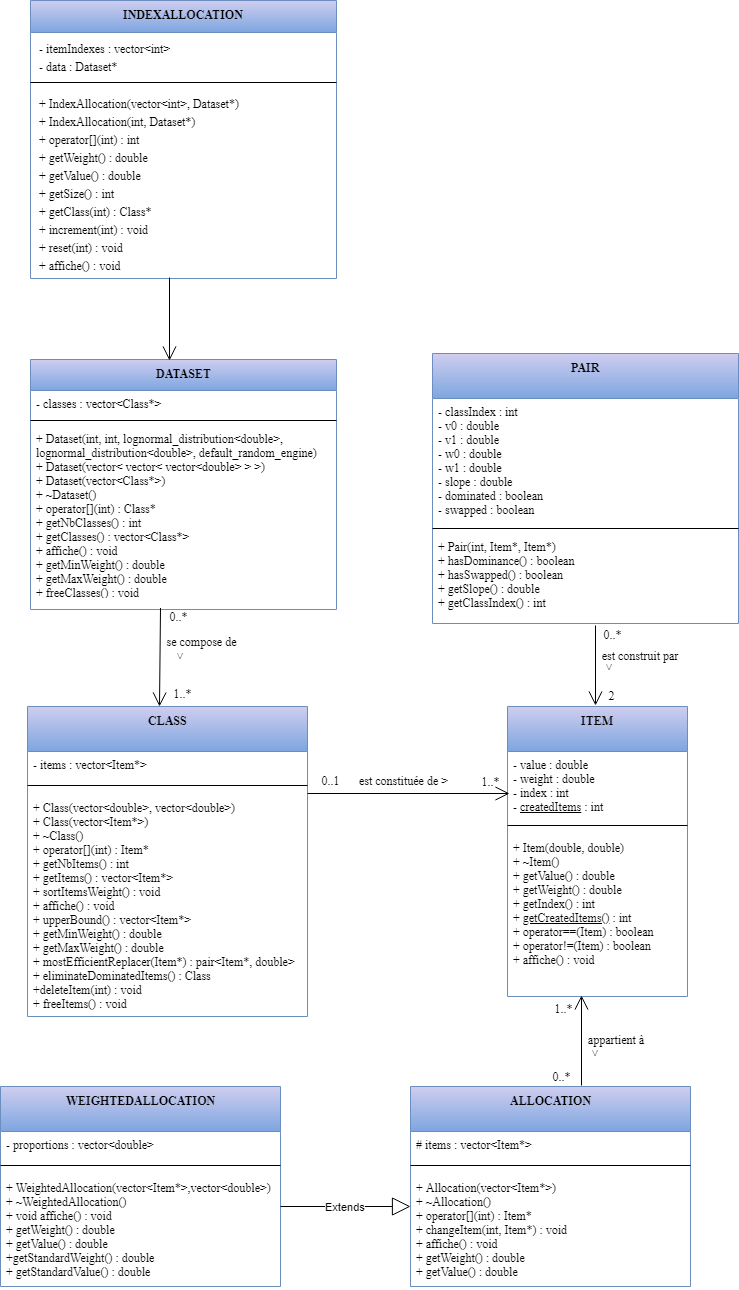
\includegraphics[width=14cm]{KnapsackClasses.png}
	\caption{Diagramme de classes}
	\label{fig:diagramme}
\end{figure}

\section{Application économique}
% Je vais ici parler de l'application du MCKP à une politique d'incitation.

Le problème du sac à dos à choix multiple peut être appliqué à la politique économique.
Considérons l'analogie suivante :
\begin{itemize}
	\item Le sac à dos représente l'économie ou un secteur de l'économie.
	\item La capacité du sac à dos représente le budget du gouvernement.
	\item Les différentes classes représente les différents individus dans l'économie.
	\item Les objets de la classe $j$ représente les choix que peux faire l'individu $j$ (par ex., choix entre plusieurs modèles de voiture, choix entre plusieurs modes de transport).
	\item La valeur de l'objet $x$ représente le bénéfice social associé au choix de $x$.
	\item Le poids de l'objet $x$ représente l'opposé de l'utilité que retire l'individu s'il fait le choix $x$ (plus le poids est faible, plus l'utilité associée est grande).
\end{itemize}

Supposons que le gouvernement utilise son budget pour distribuer des incitations aux individus de la façon suivante : si l'individu choisit $x$ mais que le gouvernement souhaite qu'il choisisse $y$ (avec $w_x < w_y$), alors le gouvernement donne une incitation d'un montant $w_y - w_x$ à l'individu pour qu'il change son choix.\footnote{Le gouvernement ayant une information parfaite sur les utilités des individus, il peut proposer l'incitation qui suffit juste à convaincre l'individu de changer son choix.}
Si l'objectif du gouvernement est de maximiser la somme des bénéfices sociaux dans l'économie, alors la solution du MCKP concorde avec la solution du programme de maximisation du gouvernement.

L'allocation optimale retournée par les algorithmes du MCKP correspond au choix qui doit être fait par chaque individus.
Le montant des incitations distribué, pour chaque individu, est égal à la différence entre le poids de l'objet choisi à l'optimum et le poids de l'objet le plus léger (c'est le choix qui procure la plus grande utilité à l'individu).

\section{Références}

\begin{thebibliography}{9}
\bibitem{Knapsack2004}
  Hans Kellerer, Ulrich Pferschy and David Pisinger,
  \textit{Knapsack problems},
  Springer,
  2004.
\end{thebibliography}

\end{document}
